\documentclass[a4paper,12pt]{article}
\usepackage[utf8]{inputenc}
\usepackage{gensymb}
\usepackage{textcomp}
\usepackage{graphicx}

%opening
\title{
  \begin{large}
    Signals \& Systems
    Assignment-5
  \end{large}
}
\author{Buncy Shaddai K \\ 17MCME08}

\begin{document}

\maketitle

  \section{Given : }
    Equation : $h_k$ = 1.62$h_{k-1}$ - 0.81$h_{k-2}$ + $\delta_k$
    \newline
    \[
    \delta_k = 
      \left\{
        \begin{array}{ll}
          1, & k = 0 \\
          0, & k \neq 0\\
        \end{array}
      \right.
    \]
    is in the form  $h_k$ = $r.p.h_{k-1}$ - $r^2$0.81$h_{k-2}$ +  $a.\delta_k$ + $b.\delta_{k-1}$
    \newline
    \hspace{40mm} where r = 0.9, p = 1.8, a = 1, b = 0

    \section{Transfer function}
      $h_k$ = 1.62$h_{k-1}$ - 0.81$h_{k-2}$ + $\delta_k$
      \newline
      $h_k$ = 1.62$h_k.z^{-1}$ - 0.81$h_k.z^{-2}$ + $\delta_k$
      \newline
      $h_k$ - 1.62$h_k.z^{-1}$ + 0.81$h_k.z^{-2}$ = $\delta_k$
      \newline
      $h_k$.(1 - 1.62$z^{-1}$ + 0.81$z^{-2}$) = $\delta_k$
      \newline
        \begin{equation}
          h_k = \frac{1}{(1 - 1.62z^{-1} + 0.81z^{-2})}\delta_k
        \end{equation}
      \hspace{36mm}  is in the form  $h_k$ = $H(z)\delta_k$
      \newline
      where $H(z)$ is a transfer function.
      \newline\newline
      By solving $1 - 1.62z^{-1} + 0.81z^{-2}$  for z, we get
      \newline
      $z = 0.81\pm\imath0.3923$

    \section{Representing in eular form}
      Writing this in terms of $e^{r\theta},$\newline
      \[
        r = \sqrt{(0.81)^2 + (0.3923)^2}
          = 0.9
      \]
      \[
        \theta = \arctan\left(\frac{0.3923}{0.81}\right)
               = 25.8419\degree
      \]
      \begin{equation}
        z = e^{(0.9).(25.8419\degree)} = 0.9(\cos(25.8419\degree)\pm\imath\sin(25.8419\degree))
      \end{equation}
    \section{Calculating frequency and no. of samples}
      The frequency of the wave is given by:
      \[
      f_n = \frac{\arccos(\frac{p}{2})}{2\pi}
      \]
      and for this problem $f_n$ is 0.0717.\newline \newline
      No. of samples =  $\left[\frac{360\degree}{\theta\degree}\right]$ = 13.9308 $\approx$ 14.

      
\pagebreak

\begin{figure}
 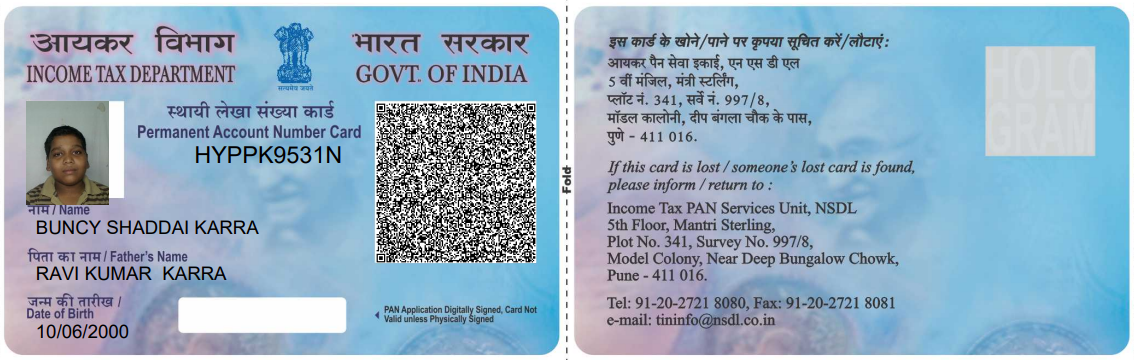
\includegraphics[scale=0.5]{panb.PNG}
\end{figure}


\end{document}
